%%%%33333
\part{Anhang}\label{part:anhang}
\frame{\partpage}

\frame{\frametitle{Anhang}\tableofcontents[part=5, hideallsubsections]}


\section{Meta-Analyse-Software für R und Stata}

\begin{frame}\frametitle{Meta-Analyse-Software für R}
  %%
  R Pakete (sozialwissenschaftliche Auswahl):
  \begin{itemize}
  \item \texttt{meta} (uni- und bivariate Meta-Analyse; mächtiger als \texttt{rmeta})
  \item \texttt{rmeta} (univariate Meta-Analyse)
  \item \texttt{metafor} (Meta-Regression; sehr umfangreich, siehe auch \url{http://www.metafor-project.org/})
  \item \texttt{mvmeta} (Multivariate Meta-Analyse)
  \item \texttt{metacor}
  \item \texttt{MAc}, \texttt{MAclinical}, \texttt{MAd} (für eine Einführung
    siehe
    \url{http://rwiki.sciviews.org/doku.php?id=packages:cran:ma_meta-analysis})
  \item \texttt{compute.es} (zur Berechnung und Konvertierung von Effektstärken)
  \end{itemize}
\end{frame}



\begin{frame}\frametitle{Meta-Analyse-Software Stata}

  \begin{itemize}
  \item Eine Liste von Stata add-ons ist unter
    \url{http://www.stata.com/support/faqs/statistics/meta-analysis/} (What
    meta-analysis features are available in Stata?) verfügbar.
  \item \citet{sterne_meta-analysis_2009} hat \enquote{Meta-Analysis in Stata:
      An Updated Collection from the Stata Journal} herausgegeben.
  \end{itemize}
\end{frame}




\begin{frame}\frametitle{Sonstige Meta-Analyse-Software}
  \begin{itemize}
   \item SPSS: "`meta-analysis stuff"' von David B. Wilson (\url{http://mason.gmu.edu/~dwilsonb/ma.html})
   \item Comprehensive Meta-Analysis: \url{http://www.meta-analysis.com/}
   \item OpenMeta[Analyst]: \url{http://tuftscaes.org/open_meta/} (interessant,
     basiert auf R und verwendet u.a. \texttt{metafor})
  \item \ldots
  \end{itemize}
\end{frame}




\section{R in 20 Minuten}

\begin{frame}[plain]\frametitle{Grundlagen von R}
  \begin{footnotesize}
    \begin{itemize}
    \item R ist ein Statistikprogramm \emph{und} eine Programmiersprache <\url{http://www.r-project.org/}>.
    \item (Fast) Alles in R sind \emph{Objekte} (etwa Datensätze oder Ergebnisse
      von Berechnungen).
    \item Sofern der Hauptspeicher ausreicht, können dort beliebig viele R
      Objekte \emph{gleichzeitig} existieren (d.h. auch mehrere Datensätze).
    \item Das Laden von Datensätzen oder Speichern von Ergebnissen ist daher
      \emph{immer} mit einer Zuweisung (\emph{assignment}) (R-Befehl: \lstinline|<-|)
      verbunden.
    \item R ist modular aufgebaut. Bestimmte (statistische) Funktionen
      (Meta-Analyse, Mehrebenenmodelle, Überlebensmodelle etc.) müssen erst (via
      \code{library(Paketname)} geladen werden.
    \item R ist \emph{case sensitive}, d.h. \texttt{mean(x)} $\neq$ \texttt{Mean(x)}.
    \item Unter MS Windows werden in R für Dateipfade immer \emph{slashes} (/)
      verwendet, \emph{backslash} ($\backslash$) ist nur als doppelter
      \emph{backslash} ($\backslash\backslash$) erlaubt.
    \item R ist streng im Umgang mit fehlenden Werten (mit \code{NA}
      gekennzeichnet) und bpsw. muss in vielen Funktionen ein listenweiser Ausschluss ausdrücklich angegeben werden.
    \item Kommentare werden mit dem Zeichen \# eingeleitet.
    \end{itemize}
  \end{footnotesize}
\end{frame}





\begin{frame}[fragile]\frametitle{Zuweisungen und R Ausgabe}

  Zuweisungen erfolgen in R mit dem Befehl \code{<-}:




\begin{knitrout}
\definecolor{shadecolor}{rgb}{0.827, 0.827, 0.827}\color{fgcolor}\begin{kframe}
\begin{alltt}
x <- 22
x
\end{alltt}
\begin{verbatim}
R> [1] 22
\end{verbatim}
\end{kframe}
\end{knitrout}


Mit \code{R>} wird hier die R-Ausgabe bezeichnet. \code{[1]} kennzeichnet in R das
i-te Elemente in der jeweiligen Zeile (hier, nur 1 Element).

\begin{knitrout}
\definecolor{shadecolor}{rgb}{0.827, 0.827, 0.827}\color{fgcolor}\begin{kframe}
\begin{alltt}
y <- 1:15
y
\end{alltt}
\begin{verbatim}
R>  [1]  1  2  3  4  5  6  7  8  9 10 11 12
R> [13] 13 14 15
\end{verbatim}
\end{kframe}
\end{knitrout}


\end{frame}



\begin{frame}[fragile, plain]\frametitle{R als Taschenrechner}
\begin{footnotesize}
\begin{knitrout}
\definecolor{shadecolor}{rgb}{0.827, 0.827, 0.827}\color{fgcolor}\begin{kframe}
\begin{alltt}
\hlcomment{## Mit Skalaren rechnen}
x <- 123
y <- 7
x + y
\end{alltt}
\begin{verbatim}
R> [1] 130
\end{verbatim}
\begin{alltt}

\hlcomment{## Mit Vektoren (= Variablen) rechnen}
\hlcomment{## c() erzeugt einen Vektor (c = concatenate)}
x <- \hlfunctioncall{c}(3, 6, 9)
x
\end{alltt}
\begin{verbatim}
R> [1] 3 6 9
\end{verbatim}
\begin{alltt}
y <- x/3
y
\end{alltt}
\begin{verbatim}
R> [1] 1 2 3
\end{verbatim}
\end{kframe}
\end{knitrout}

\end{footnotesize}
\end{frame}



\begin{frame}\frametitle{Wichtige Funktionen}
  \begin{itemize}
  \item Hilfeseiten aufrufen: \code{help(Funktionsname)} oder
    \code{?Funktionsname} (Bsp.: \code{help(mean)} oder \code{?mean})
  \item Welche Objekte sind im \emph{workspace}: \code{ls()}
  \item Arbeitsverzeichnis definieren/abfragen: \code{setwd("Pfad")} und \code{getwd()}
  \item Beschreibung eines R-Objektes: \code{str(Robjekt)}
  \item (Variablen-)Namen eines R-Objektes: \code{names(Robjekt)}
  \item Die ersten n Fälle anzeigen: \code{head(Robjekt)}
  \end{itemize}
\end{frame}


\begin{frame}[plain, fragile, shrink=10]\frametitle{Hilfeausgabe für \code{?mean}}

\begin{tiny}
\begin{verbatim}
mean                   package:base                    R Documentation

Arithmetic Mean

Description:

     Generic function for the (trimmed) arithmetic mean.

Usage:

     mean(x, ...)

     ## Default S3 method:
     mean(x, trim = 0, na.rm = FALSE, ...)

Arguments:

       x: An R object.  Currently there are methods for numeric/logical
          vectors and date, date-time and time interval objects, and
          for data frames all of whose columns have a method.  Complex
          vectors are allowed for ‘trim = 0’, only.

    trim: the fraction (0 to 0.5) of observations to be trimmed from
          each end of ‘x’ before the mean is computed.  Values of trim
          outside that range are taken as the nearest endpoint.

   na.rm: a logical value indicating whether ‘NA’ values should be
          stripped before the computation proceeds.

     ...: further arguments passed to or from other methods.

Value:

     If ‘trim’ is zero (the default), the arithmetic mean of the values
     in ‘x’ is computed, as a numeric or complex vector of length one.
     If ‘x’ is not logical (coerced to numeric), numeric (including
     integer) or complex, ‘NA_real_’ is returned, with a warning.

     If ‘trim’ is non-zero, a symmetrically trimmed mean is computed
     with a fraction of ‘trim’ observations deleted from each end
     before the mean is computed.

References:

     Becker, R. A., Chambers, J. M. and Wilks, A. R. (1988) _The New S
     Language_.  Wadsworth & Brooks/Cole.

See Also:

     ‘weighted.mean’, ‘mean.POSIXct’, ‘colMeans’ for row and column
     means.

Examples:

     x <- c(0:10, 50)
     xm <- mean(x)
     c(xm, mean(x, trim = 0.10))
\end{verbatim}
\end{tiny}
\end{frame}



\begin{frame}[fragile]\frametitle{Daten laden und untersuchen I}
\begin{footnotesize}



\begin{knitrout}
\definecolor{shadecolor}{rgb}{0.827, 0.827, 0.827}\color{fgcolor}\begin{kframe}
\begin{alltt}
\hlcomment{## Zuweisung nicht vergessen!}
dat <- \hlfunctioncall{read.csv}(file = \hlstring{"../../data/dVerbAb.csv"},
                sep = \hlstring{";"}, dec = \hlstring{","})

\hlcomment{## head() zeigt die ersten 6 Zeilen eines}
\hlcomment{## R Objektes an}
\hlfunctioncall{head}(dat)
\end{alltt}
\begin{verbatim}
R>   ID year pub     r   N      Var      SE
R> 1  1 1980   0 -0.10   7 0.163350 0.40417
R> 2  2 2005   1  0.23  76 0.011960 0.10936
R> 3  4 1968   0 -0.05 155 0.006461 0.08038
R> 4  5 1968   0  0.02  45 0.022709 0.15070
R> 5  6 1969   1 -0.09  31 0.032796 0.18110
R> 6  7 1969   1  0.26  37 0.024149 0.15540
\end{verbatim}
\end{kframe}
\end{knitrout}

\end{footnotesize}
\end{frame}


\begin{frame}[fragile, plain]\frametitle{Daten laden und untersuchen II}
\begin{tiny}

\begin{knitrout}
\definecolor{shadecolor}{rgb}{0.827, 0.827, 0.827}\color{fgcolor}\begin{kframe}
\begin{alltt}
\hlcomment{## Struktur anzeigen}
\hlfunctioncall{str}(dat)
\end{alltt}
\begin{verbatim}
R> 'data.frame':	17 obs. of  7 variables:
R>  $ ID  : int  1 2 4 5 6 7 9 10 11 12 ...
R>  $ year: int  1980 2005 1968 1968 1969 1969 1970 1987 1987 1993 ...
R>  $ pub : int  0 1 0 0 1 1 0 1 1 1 ...
R>  $ r   : num  -0.1 0.23 -0.05 0.02 -0.09 0.26 -0.07 0.04 -0.01 0.12 ...
R>  $ N   : int  7 76 155 45 31 37 79 151 151 64 ...
R>  $ Var : num  0.16335 0.01196 0.00646 0.02271 0.0328 ...
R>  $ SE  : num  0.4042 0.1094 0.0804 0.1507 0.1811 ...
\end{verbatim}
\begin{alltt}

\hlcomment{## Dimensionen}
\hlfunctioncall{dim}(dat)
\end{alltt}
\begin{verbatim}
R> [1] 17  7
\end{verbatim}
\begin{alltt}

\hlcomment{## Variablennamen ausgeben lassen}
\hlfunctioncall{names}(dat)
\end{alltt}
\begin{verbatim}
R> [1] "ID"   "year" "pub"  "r"    "N"    "Var" 
R> [7] "SE"
\end{verbatim}
\end{kframe}
\end{knitrout}

\end{tiny}
\end{frame}


\begin{frame}[fragile]\frametitle{Mit Datenobjekten (data.frame) arbeiten I}
\begin{footnotesize}
\begin{knitrout}
\definecolor{shadecolor}{rgb}{0.827, 0.827, 0.827}\color{fgcolor}\begin{kframe}
\begin{alltt}
\hlcomment{## Einzelne Elemente eines data.frame}
\hlcomment{## ansprechen: mit $}
dat$r
\end{alltt}
\begin{verbatim}
R>  [1] -0.10  0.23 -0.05  0.02 -0.09  0.26 -0.07
R>  [8]  0.04 -0.01  0.12  0.03  0.07 -0.05  0.13
R> [15]  0.03  0.21  0.28
\end{verbatim}
\begin{alltt}

\hlcomment{## Einzelne Elemente des data.frame}
\hlcomment{## ansprechen: Indexnotation}
dat[, \hlstring{"r"}]
\end{alltt}
\begin{verbatim}
R>  [1] -0.10  0.23 -0.05  0.02 -0.09  0.26 -0.07
R>  [8]  0.04 -0.01  0.12  0.03  0.07 -0.05  0.13
R> [15]  0.03  0.21  0.28
\end{verbatim}
\end{kframe}
\end{knitrout}

\end{footnotesize}
\end{frame}


\begin{frame}[fragile]\frametitle{Mit Datenobjekten (data.frame) arbeiten II}
\begin{footnotesize}
\begin{knitrout}
\definecolor{shadecolor}{rgb}{0.827, 0.827, 0.827}\color{fgcolor}\begin{kframe}
\begin{alltt}
\hlcomment{## Mehrere Elemente eines data.frame}
\hlcomment{## ansprechen: nur noch Indexnotation}
\hlcomment{## Fälle 1:5, Variablen: r und Var}
dat[1:5, \hlfunctioncall{c}(\hlstring{"r"}, \hlstring{"Var"})]
\end{alltt}
\begin{verbatim}
R>       r      Var
R> 1 -0.10 0.163350
R> 2  0.23 0.011960
R> 3 -0.05 0.006461
R> 4  0.02 0.022709
R> 5 -0.09 0.032796
\end{verbatim}
\end{kframe}
\end{knitrout}

\end{footnotesize}
\end{frame}


\begin{frame}[fragile, plain]\frametitle{Deskriptive Statistik}
\begin{footnotesize}
\begin{knitrout}
\definecolor{shadecolor}{rgb}{0.827, 0.827, 0.827}\color{fgcolor}\begin{kframe}
\begin{alltt}
\hlfunctioncall{summary}(dat[, \hlfunctioncall{c}(\hlstring{"r"}, \hlstring{"pub"})])
\end{alltt}
\begin{verbatim}
R>        r                pub       
R>  Min.   :-0.1000   Min.   :0.000  
R>  1st Qu.:-0.0500   1st Qu.:0.000  
R>  Median : 0.0300   Median :1.000  
R>  Mean   : 0.0618   Mean   :0.706  
R>  3rd Qu.: 0.1300   3rd Qu.:1.000  
R>  Max.   : 0.2800   Max.   :1.000
\end{verbatim}
\begin{alltt}
\hlfunctioncall{sd}(dat$r)
\end{alltt}
\begin{verbatim}
R> [1] 0.1241
\end{verbatim}
\begin{alltt}
\hlfunctioncall{table}(dat$pub)
\end{alltt}
\begin{verbatim}
R> 
R>  0  1 
R>  5 12
\end{verbatim}
\end{kframe}
\end{knitrout}

\end{footnotesize}
\end{frame}



\begin{frame}[fragile]\frametitle{Einen Teildatensatz erstellen}\framesubtitle{SPSS/Stata: \code{if}}
\begin{footnotesize}
\begin{knitrout}
\definecolor{shadecolor}{rgb}{0.827, 0.827, 0.827}\color{fgcolor}\begin{kframe}
\begin{alltt}
\hlfunctioncall{subset}(dat, pub==0)
\end{alltt}
\begin{verbatim}
R>    ID year pub     r   N      Var      SE
R> 1   1 1980   0 -0.10   7 0.163350 0.40417
R> 3   4 1968   0 -0.05 155 0.006461 0.08038
R> 4   5 1968   0  0.02  45 0.022709 0.15070
R> 7   9 1970   0 -0.07  79 0.012695 0.11267
R> 11 13 1991   0  0.03 318 0.003149 0.05612
\end{verbatim}
\begin{alltt}
\hlfunctioncall{subset}(dat, pub==0 & r > 0)
\end{alltt}
\begin{verbatim}
R>    ID year pub    r   N      Var      SE
R> 4   5 1968   0 0.02  45 0.022709 0.15070
R> 11 13 1991   0 0.03 318 0.003149 0.05612
\end{verbatim}
\end{kframe}
\end{knitrout}

\end{footnotesize}
\end{frame}



\begin{frame}[fragile]\frametitle{Bedingtes Recodieren}
\begin{footnotesize}
\begin{knitrout}
\definecolor{shadecolor}{rgb}{0.827, 0.827, 0.827}\color{fgcolor}\begin{kframe}
\begin{alltt}
\hlcomment{## Kopie erstellen}
tmp <- dat
tmp$pub
\end{alltt}
\begin{verbatim}
R>  [1] 0 1 0 0 1 1 0 1 1 1 0 1 1 1 1 1 1
\end{verbatim}
\begin{alltt}

\hlcomment{## pub == 0 mit 99 ersetzen}
tmp$pub <- \hlfunctioncall{ifelse}(tmp$pub == 0, 99, tmp$pub)
tmp$pub
\end{alltt}
\begin{verbatim}
R>  [1] 99  1 99 99  1  1 99  1  1  1 99  1  1  1  1
R> [16]  1  1
\end{verbatim}
\end{kframe}
\end{knitrout}

\end{footnotesize}
\end{frame}


\begin{frame}[fragile, plain, shrink]\frametitle{Umgang mit Missings}
\begin{footnotesize}
\begin{knitrout}
\definecolor{shadecolor}{rgb}{0.827, 0.827, 0.827}\color{fgcolor}\begin{kframe}
\begin{alltt}
\hlcomment{## Kopie erstellen}
tmp <- dat
\hlcomment{## 0 wird zu missing (NA)}
tmp$pub <- \hlfunctioncall{ifelse}(tmp$pub == 0, NA, tmp$pub)

\hlcomment{## subset nur missings in pub}
\hlfunctioncall{subset}(tmp, \hlfunctioncall{is.na}(pub))
\end{alltt}
\begin{verbatim}
R>    ID year pub     r   N      Var      SE
R> 1   1 1980  NA -0.10   7 0.163350 0.40417
R> 3   4 1968  NA -0.05 155 0.006461 0.08038
R> 4   5 1968  NA  0.02  45 0.022709 0.15070
R> 7   9 1970  NA -0.07  79 0.012695 0.11267
R> 11 13 1991  NA  0.03 318 0.003149 0.05612
\end{verbatim}
\begin{alltt}

\hlcomment{## is.na-Funktion}
\hlfunctioncall{is.na}(tmp$pub)
\end{alltt}
\begin{verbatim}
R>  [1]  TRUE FALSE  TRUE  TRUE FALSE FALSE  TRUE
R>  [8] FALSE FALSE FALSE  TRUE FALSE FALSE FALSE
R> [15] FALSE FALSE FALSE
\end{verbatim}
\end{kframe}
\end{knitrout}

\end{footnotesize}
\end{frame}




\begin{frame}[plain]\frametitle{RStudio und R}
  \begin{itemize}
  \item Unter MS-Windows gibt es zur Bedienung von R nur die spartanische R Console.
  \item Empfehlenswert ist RStudio, eine kostenlose integrierte
    Entwicklungsumgebung für R <\url{http://www.rstudio.com/ide/}>.
  \end{itemize}
  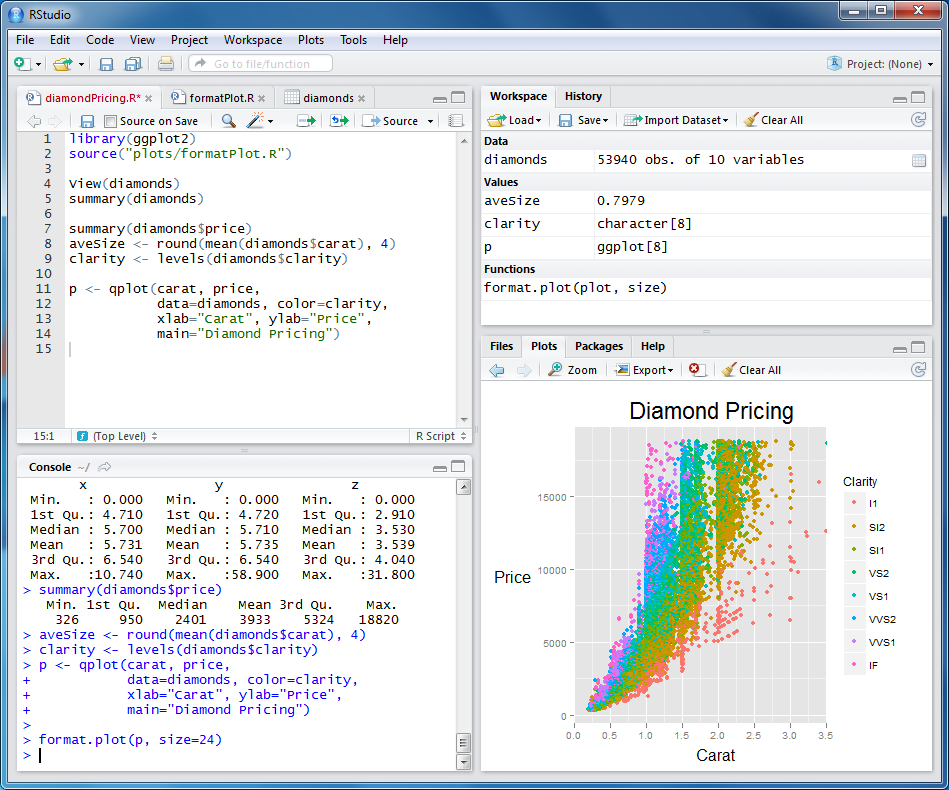
\includegraphics[width=0.7\textwidth]{rstudio-windows.png}
\end{frame}


\section{Statistische Grundlagen}


\subsection{Der Standardfehler}\label{sec:der-standardfehler}

\begin{frame}
  \frametitle{Was ist Inferenzstatistik?}
  \begin{itemize}
  \item<+-> Inferenzstatistik befasst sich mit dem Schluss von der Stichprobe auf die Grundgesamtheit (Population).
  \item<+-> Dieser Schluss ist (immer) fehlerbehaftet; neben dem Schätzen des Populationsparameters ("`Punktschätzung"') ist daher von
    zentraler Bedeutung, die Unsicherheit bei der Parameterschätzung beschreiben zu können.
  \item<+-> Der \emph{Standardfehler} ist ein Streuungsmaß, das die Unsicherheit der Parameterschätzung beschreibt.
  \item<+-> Mit Hilfe des Standardfehlers lässt sich das Konfidenzintervall ("`Intervallschätzung"') berechnen sowie die
    Irrtumswahrscheinlichkeit bestimmen.
  \end{itemize}
\end{frame}


\begin{frame}
  \frametitle{Der Standardfehler für das arithmetische Mittel}
  \begin{itemize}
      \item Der SE beschreibt die Güte des ermittelten Stichprobenwertes: Je größer die Fallzahl, desto kleiner der
    SE. Je kleiner der Standardfehler, desto besser die Schätzung.
  \item Der Standardfehler (SE) des Stichprobenmittelwertes lautet:
    \begin{equation*}
      \frac{\text{Standardabweichung des Merkmals}}{\sqrt{\text{Fallzahl}}}=\frac{\sigma}{\sqrt{N}}.
    \end{equation*}
  \item Der SE gibt die Streuung der Stichproben-Mittelwerte von gleichgroßen und zufällig aus einer Grundgesamtheit gezogenen
    Stichproben um den wahren Populationsmittelwert $\mu$ (sprich "`mü"'; allgemein: $\theta$, sprich: theta) an.
  \end{itemize}
\end{frame}

\subsection{Wahrscheinlichkeitsverteilungen und Q-Test}


\begin{frame}
  \frametitle{Exkurs: Die statistische Beschreibung von Wahrscheinlichkeitsverteilungen}
  Die folgenden Ausführungen zur statistischen Signifikanz von Q verweisen (teilweise implizit, teilweise explizit) auf
  die Beschreibung der Wahrscheinlichkeitsverteilung einer Zufallsvariablen. Die folgenden Begriffe sollten Sie ggf. noch einmal auffrischen:
  \begin{itemize}
  \item Diskrete Zufallsvariablen: Wahrscheinlichkeitsfunktion; stetige Zufallsvariablen:
    Wahrscheinlichkeitsdichtefunktion (teilw. mit "`Dichte"' abgekürzt; engl.: \emph{probability density function})
  \item Mit Hilfe von Wahrscheinlichkeitsverteilungen lassen sich Ereignissen Wahrscheinlichkeiten zuordnen.
  \item (Kumulative) Verteilungsfunktion
  \item Quantilfunktion
  \end{itemize}
\end{frame}



\begin{frame}
  \frametitle{Idee des $Q$-Tests (I)}
  %%
  \begin{itemize}
  \item $Q$ ist die Gesamtvariation (nicht -varianz!) (beobachtete Variation), $df = k-1$ die erwartete Variation im
    Falle des FEM (es gibt \emph{einen gemeinsamen} Populationsparameter) und $Q-k-1$ die Abweichung zwischen
    beobachteter und erwarteter Variation.
  \item Wenn $Q \leq df$ gilt, dann wird definitionsgemäß $Q=0$ und es wird eine homogene Effektstärkenverteilung
    unterstellt.
  \item Wenn aber $Q > df$ ($Q-df > 0$) gilt, müssen wir dann \emph{immer} von einer heterogenen ES-Verteilung ausgehen? Oder
    muss $Q$ ($Q-df$) nicht "'ziemlich groß sein"', damit die Idee einer homogenen Effektstärkenverteilung zurückgewiesen
    werden kann? Was aber heißt "`ziemlich groß"'?
  \end{itemize}
\end{frame}


\begin{frame}[plain]
  \frametitle{Idee des $Q$-Tests (II)}
  %%
  \begin{small}
    \begin{itemize}
    \item Der $Q$-Wert folgt einer sogenannten $\chi^2$-Verteilung (gehört zu den stetigen
      Wahrscheinlichkeitsverteilungen).
    \item Mit dem Wissen, dass $Q$ $\chi^2$-verteilt ist, lässt sich für einen gegebenen Freiheitsgrad ($df$) bspw. die
      Wahrscheinlichkeit $Pr(0 \leq Q)$ bestimmten, d.h., dass ein bestimmter $Q$-Wert im Intervall $[0, Q]$ liegt. Die
      Wahrscheinlichkeit, dass $Q$ außerhalb des Intervalls liegt (also größer als $Q$ ist bzw. $(Q; +\infty]$), beträgt
      $1-Pr(0 \leq Q)$. Anders formuliert: $1-Pr(0 \leq Q)$ ist die Wahrscheinlichkeit, einen Wert größer als $Q$ zu bekommen.
    \item "`Ziemlich groß"' (siehe vorherige Folie) ist ein $Q$-Wert aber doch dann, wenn $1-Pr(0 \leq Q)$ (= p-Wert =
      Irrtumswahrscheinlichkeit) klein ist, wobei
      verschiedene "`Kleinheitsgrade"' (10\%, 5\%, 1\% = Signifikanzniveaus) unterschieden werden. Zu jedem dieser
      Signifikanzniveaus lässt sich ein theoretischer $\chi^2$-Wert berechnen und wenn der empirische $\chi^2$-Wert (als
      $Q$) größer ist, dann sagen wir, dass der Wert signifikant auf dem 10\%-, 5\%-, 1\%-Niveau ist.
    \item Üblicherweise wird in der Meta-Analyse-Literatur das 10\%-Niveau angenommen.
    \end{itemize}
  \end{small}
\end{frame}


\begin{frame}[fragile, plain]
  \frametitle{Bestimmung der Irrtumswahrscheinlichkeit von $Q$}
  %%
\begin{footnotesize}
Mit R lässt sich für verschiedene Wahrscheinlichkeitsverteilungen die Wahrscheinlichkeit $Pr(X \leq x)$ (= F(x) =
kumulative Verteilungsfunktion) bestimmten -- und nur diese. Da im Falle des Q-Testes aber $1-Pr(0 \leq Q)$ = p-Wert
gesucht wird, muss folglich immer $1-Pr(0 \leq
Q)$ gerechnet werden.

%%berechnungChisq, keep.source = TRUE
\begin{knitrout}
\definecolor{shadecolor}{rgb}{0.827, 0.827, 0.827}\color{fgcolor}\begin{kframe}
\begin{alltt}
\hlcomment{## Q = 10 (df = 5)}
1-\hlfunctioncall{pchisq}(q = 10, df = 5)
\end{alltt}
\begin{verbatim}
R> [1] 0.07524
\end{verbatim}
\begin{alltt}

\hlcomment{## Q = 36.1437 (df = 5), Borenstein Tab 14.7}
1-\hlfunctioncall{pchisq}(q = 36.1437, df = 5)
\end{alltt}
\begin{verbatim}
R> [1] 8.89e-07
\end{verbatim}
\begin{alltt}

\hlcomment{## Welches Q fuer alpha <= 0.1?}
\hlfunctioncall{qchisq}(0.9, df  = 5)
\end{alltt}
\begin{verbatim}
R> [1] 9.236
\end{verbatim}
\end{kframe}
\end{knitrout}

\end{footnotesize}
\end{frame}


\begin{frame}[shrink = 5]
  \frametitle{Quantile der $\chi^2-Verteilung$ (df = 3)}
  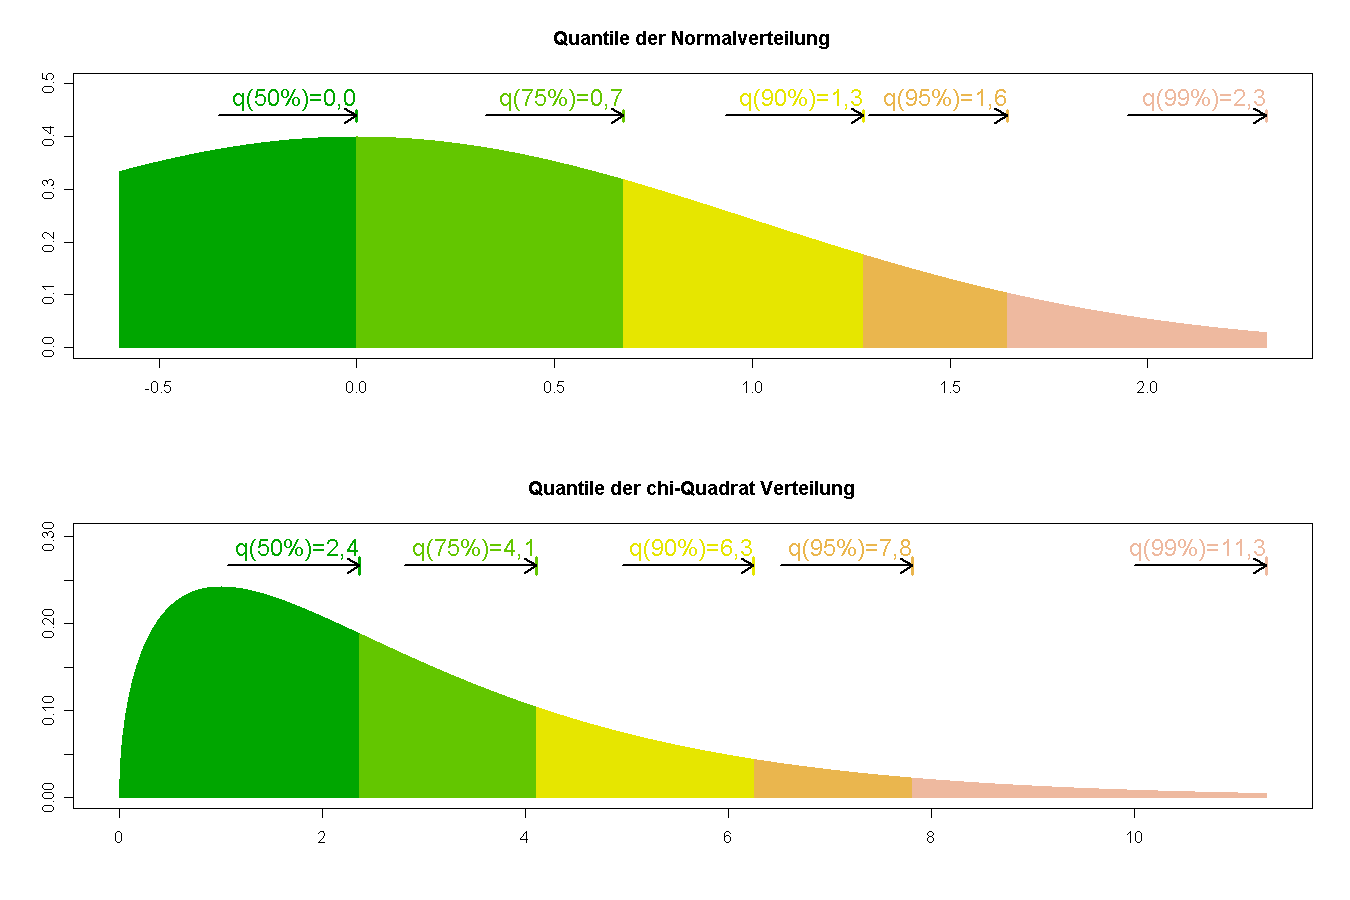
\includegraphics[width=0.9\textwidth]{Quantile_graph}
\newline(Quelle: \url{http://de.wikipedia.org/wiki/Chi-Quadrat-Verteilung})
\end{frame}





%%% Local Variables:
%%% mode: latex
%%% TeX-master: "ps2012gesis-ma-workshop.Rnw"
%%% End:
